% !TEX root = tracking.tex
\section{Offline Computations \label{sec:precomp}}

To precompute the tracking bound we set up a capture-avoid game between the real and virtual vehicles, which we then analyze using HJ reachability. In this game, the real system will try to "capture" the virtual system, while the virtual system is doing everything it can to avoid capture. By using reachability to analyze this game we will get a guaranteed bound on how far apart the two vehicles will ever be even when the virtual system is acting as inconveniently as possible.

\subsection{Relative Dynamics}
The states and dynamics of the real system, as defined in section \ref{sec:formulation}, are $\dot\tstate = \tdyn(\tstate, \tctrl, \dstb)$. The virtual system will have states $\vstate$, which we assume to be a subset of $\tstate$. The virtual system has dynamics $\dot\vstate = \vdyn(\vstate, \vctrl)$, with control $\vctrl$.
\SHnote{restrictions on $vctrl$?}

\textcolor{red}{introduce virtual dynamics, explain that it must be a subset of real system dynamics}
We now have the dynamics for the individual systems, but to set up the capture-avoid game we must first define the relative states and dynamics. We place the virtual vehicle at the origin by subtracting its states $(\vstate)$ from the real system's states $(\tstate)$. In this frame of reference $(\rstate)$ we are given the states of the real system relative to the virtual system. \textcolor{red}{incorporate disturbances here?}


\MCnote{I copied some old writing here. We should choose a common set of commands for stuff like real state and virtual state.}

Dynamics of system
\begin{equation}
\dot\vstate = \vdyn(\vstate, \vctrl, \dstb)
\end{equation}

Dynamics of trajectory

\begin{equation}
\begin{aligned}
\rstate = \tstate - \tvmat\vstate\\
\dot\rstate = \rdyn(\rstate, \tctrl, \vctrl, \dstb)
\end{aligned}
\end{equation}

Matrix $\tvmat$ matches the common states of $\tstate$ and $\vstate$. The states $\rstate$ now represent the real state relative to the virtual state.

\MCnote{I copied some old writing here. We should choose a common set of commands for stuff like real state and virtual state.}
\MCnote{$\tvmat$ is a matrix that subsamples the states. It could be a more general transformation which would be useful for doing rotations (eg. in air3D there's also rotation so that one vehicle is facing right)}


Tracking error: $\rstate {\tvind}$.

Define an error function $\errfunc(\rstate)$

We now have the dynamics for the individual systems, but to set up the capture-avoid game we must first define the relative states and dynamics. We place the virtual vehicle at the origin by subtracting its states $(z_2)$ from the real system's states $(z_1)$. In this frame of reference $(z_r)$ we are given the states of the real system relative to the virtual system. \textcolor{red}{incorporate disturbances here?}

\MCnote{Yes, we should always incorporate disturbances for the real system dynamics. I think the relative dynamics needs the $\tvmat$ matrix though, otherwise subtraction wouldn't make sense.}

\begin{equation}
\dot\vstate = \vdyn(\vstate, \vctrl, \dstb)
\end{equation}

Dynamics of trajectory
\begin{equation}
\dot\tstate = \tdyn(\tstate, \tctrl)
\end{equation}

Assume $\tstate$ is a subset of $\vstate$. 

Relative state:
\begin{equation}
\rstate = \vstate - \tvmat\tstate
\end{equation}

Relative dynamics
\begin{equation}
\dot\rstate = \rdyn(\rstate, \vctrl, \tctrl, \dstb)
\end{equation}

The relative dynamics will include the relative position states and any other relevant states such as relative angles and velocities.

\subsection{Formalizing the Capture-Avoid Game}
\MCnote{The goal of the system is to minimize the tracking error. The goal of the trajectory, which is a ``virtual'' vehicle, is to maximize the tracking error. (copied from old writing)}

Now that we have the relative dynamics between the two systems we must define a metric for the tracking error bound between these systems. We do this by defining an implicit surface function as a reward function $l(\rstate)$ in the new frame of reference \SHnote{requirements on $l(\rstate)$} Because the metric we care about is distance to the origin, this reward function can be as simple as negative distance in position space to the origin. An example can be seen in Figure \ref{fig:quad4D_example}-a, where the rings represent varying level sets of the cost function. The real vehicle will try to maximize this reward to reduce the relative distance, while the virtual vehicle will do the opposite.

\begin{figure}
	\centering
	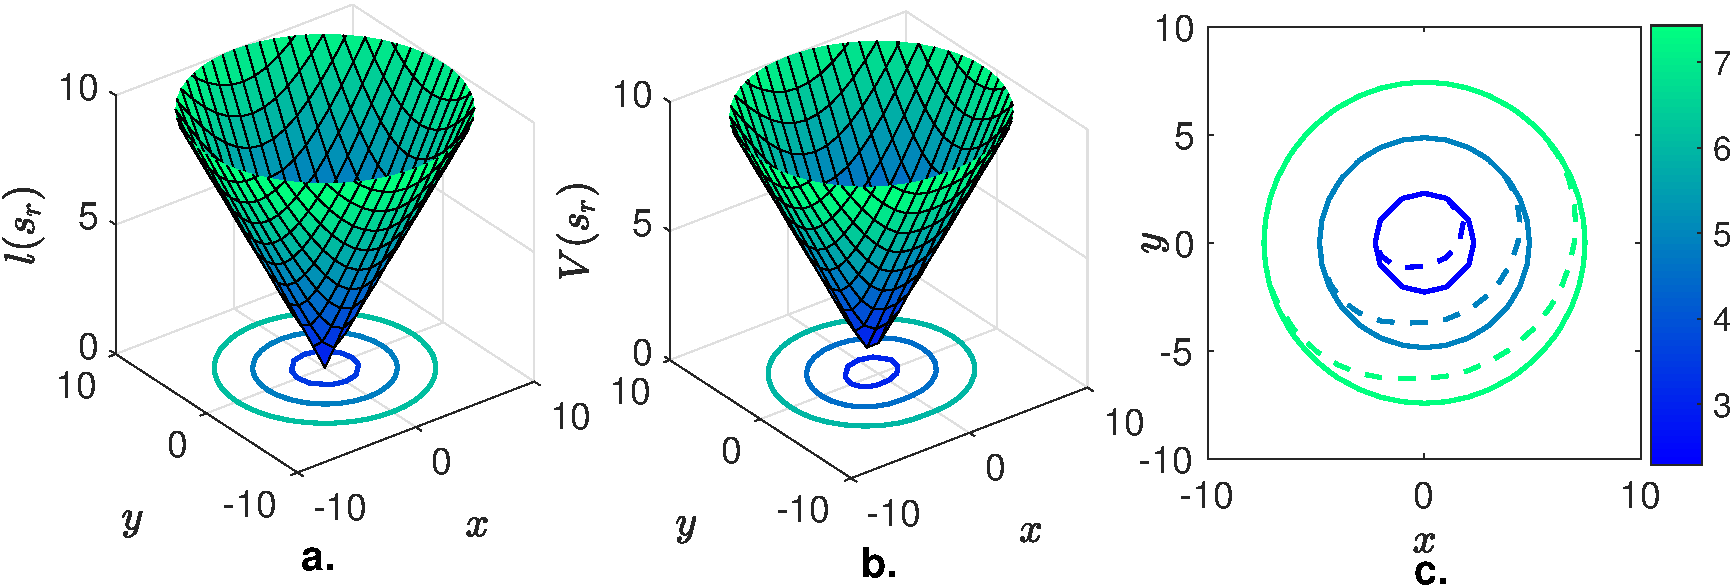
\includegraphics[width=0.5\textwidth]{fig/quad4D_example}
	\caption{\textcolor{red}{a) reward function, b) value function, c) level sets of both mapping initial state to tracking error bound}}
	\label{fig:quad4D_example}
\end{figure} 
 
 We want to find the farthest distance (and thus highest cost) that this game will ever reach when both players are acting optimally. Therefore we want to find a mapping between the initial state of the system and the maximum cost achieved over the time horizon. This mapping is through our value function, defined as: \MCnote{Time horizon, time variable notation, control/disturbance functions, trajectory notation}
 \begin{equation}
 \begin{aligned}
 	V(\rstate)= \min_{\vctrl} \max_{\tctrl} \max_{t\in [0,T]} l(\state_r(\tau)), \ \tau \in [t, 0]
 	\end{aligned}
 \end{equation} 
 
 This is a modified version of the Hamilton-Jacobi formulation as described by \textcolor{red}{cite jaime, time varying reachability}. By implementing reachability analysis we solve for this value function over the time horizon. If the control authority of the real system is powerful enough to always eventually reach the virtual system, this value function will converge to an invariant solution for all time.  An example of this value function is in Figure \ref{fig:quad4D_example}-b. In the next section we will prove that the sub-level sets of this value function will map initial relative states to the guaranteed furthest possible tracking error over all time, as seen in Figure \ref{fig:quad4D_example}-c.
 
\subsection{Main Result}

 \begin{equation}
 \begin{aligned}
& \valfunc(\rstate, \thor) = \max_{\vctrl(\cdot)} \min_{\tctrl(\cdot), \dstb(\cdot)} \big\{\\
&\quad \min_{\tvar \in [-\thor, 0]} \errfunc(\rtraj(\tvar; \rstate, -\thor, \vctrl(\cdot), \tctrl(\cdot), \dstb(\cdot)))\big\} 
 \end{aligned}
  \end{equation}
 
 \begin{thm}
   \label{thm:main}
   Let $\thor_c \ge 0$, and suppose
   
   \begin{equation}
   \label{eq:conv_valfunc}
   \valfunc_\infty(\rstate) := \valfunc(\rstate, \thor) = \valfunc(\rstate, \thor_c) ~ \forall \thor \ge \thor_c.
   \end{equation}
   
   Then $\forall \tvar_1, \tvar_2$ with $\tvar_1 \ge \tvar_2$,
   
   \begin{equation}
   \valfunc_\infty\Big(\rtraj(\tvar_2; \rstate, \tvar_1, \vctrl^*(\cdot), \tctrl^*(\cdot), \dstb^*(\cdot))\Big) \ge \valfunc_\infty(\rstate)
   \end{equation}
   
   \noindent where
   \begin{equation}
   \begin{aligned}
   & \vctrl^*(\cdot) = \arg \max_{\vctrl(\cdot)} \min_{\tctrl(\cdot), \dstb(\cdot)}\big\{ \\
   & \qquad \min_{\tvar \in [-\thor_1, 0]} \errfunc(\rtraj(0; \rstate, \tvar, \vctrl(\cdot), \tctrl(\cdot), \dstb(\cdot))) \big\}\\
   & \tctrl^*(\cdot) = \arg \min_{\tctrl(\cdot)} \min_{\dstb(\cdot)} \big\{ \\
   & \qquad \min_{t \in [-\thor_1, 0]} \errfunc(\rtraj(0; \rstate, \tvar, \vctrl(\cdot), \tctrl(\cdot), \dstb(\cdot))) \big\} \\
   & \dstb^*(\cdot) = \arg \min_{\dstb(\cdot)} \big\{\min_{\tvar \in [-\thor_1, 0]} \errfunc(\rtraj(0; \rstate, \tvar, \vctrl(\cdot), \tctrl(\cdot),  \dstb(\cdot))) \big\}
   \end{aligned}
   \end{equation}
   
 \end{thm}
 
\textit{Proof:} For convenience, let

\begin{equation}
\rtraj^*(0;, \rstate, \tvar) := \rtraj(0; \rstate, \tvar, \vctrl^*(\cdot), \tctrl^*(\cdot), \dstb^*(\cdot)))
\end{equation}

First, we break up the expression ``$\min_{\tvar \in [-\thor, 0]}$'' into two parts with time intervals $[-\thor_c, 0], [-\thor, -\thor_c]$. For all $\thor \ge \thor_c$,
   
   \begin{equation}
   \begin{aligned}
   \valfunc(\rstate, \thor) &= \min_{\tvar \in [-\thor, 0]} \errfunc(\rtraj^*(\tvar; \rstate, -\thor)) \\
   &= \min \Big[ \min_{\tvar \in [-\thor_c, 0]} \errfunc(\rtraj^*(\tvar; \rstate, -\thor)), \\
   &\qquad\qquad\min_{\tvar \in [-\thor, -\thor_c]} \errfunc(\rtraj^*(\tvar; \rstate, -\thor)) \Big]
   \end{aligned}
   \end{equation}
   
   Next, using \eqref{eq:conv_valfunc}, we have
   \begin{equation}
   \begin{aligned}
   \valfunc_\infty(\rstate) &= \min \Big[ \valfunc_\infty(\rtraj^*(-\thor_c; \rstate, -\thor)), \\
   &\qquad\qquad\min_{\tvar \in [-\thor, -\thor_c]} \errfunc(\rtraj^*(\tvar; \rstate, -\thor)) \Big]
   \end{aligned}
   \end{equation}
   
   \noindent which trivially implies
   \begin{equation}
   \valfunc_\infty(\rstate) \le \valfunc_\infty(\rtraj^*(-\thor_c; \rstate, -\thor))
   \end{equation}
   
   Since the system dynamics are time-invariant, we can pick $\tvar_2 = -\thor_c$ without loss of generality, and $\tvar_1 = -\thor$ to obtain the desired result. \hfill $\blacksquare$
 
 \textit{Remark:} Theorem \ref{thm:main} is a well-known result in differential game theory \cite{}, and has been utilized in the context of using the subzero level set of $\valfunc_\infty$ as a backward reachable set for tasks such as collision avoidance or reach-avoid games \cite{}. 
